\documentclass[11pt]{beamer}
\usetheme{Luebeck}
%\usecolortheme{seahorse}
\useinnertheme{rectangles}
\useoutertheme{infolines}
\usepackage{xcolor}
\usepackage{natbib}
\usepackage[utf8]{inputenc}
\usepackage{tikz}
\usepackage{tabularx}
\usepackage{lipsum}
\usepackage{amsmath,graphicx,dsfont}
\usepackage{graphicx}
\usetikzlibrary{shapes,backgrounds,arrows,automata,snakes,shadows,positioning, mindmap}
%\usepackage[citestyle=verbose]{biblatex}
%===================================
\newcommand\betab{{\boldsymbol{\beta}}}
\newcommand\thetab{{\boldsymbol{\theta}}}
\newcommand\Sigmab{{\boldsymbol{\Sigma}}}
\newcommand\Yb{{\bf Y}}
\newcommand\Zb{{\bf Z}}
%===================================
\newcommand{\Ccal}{\mathcal{C}}
\newcommand{\edgeunit}{1.5}
\newcommand{\smalledgeunit}{1}
\newcommand{\emphase}[1]{\textcolor{Complement}{#1}}
\newcommand{\bleu}[1]{\textcolor{Framableulight}{#1}}
\newcommand{\pos}[1]{\textcolor{Darkgreen}{#1}}
\newcommand{\nega}[1]{\textcolor{Nicered}{#1}}
\newcommand{\independent}{\perp \!\!\! \perp}

\newcommand{\Ncal}{\mathcal{N}}
\tikzset{%
    observed/.style={%
    scale=0.6,circle,draw=Framableulight,transform shape,fill=white,font=\Large}
}
\tikzset{%
    bigMissing/.style={%
    scale=0.6,circle,draw=orange,transform shape,fill=white,font=\Large}
}
\tikzset{%
    basic/.style={%
    scale=0.4,circle,draw=Framableu,transform shape,fill=Framableulight,font=\small}
}
\tikzset{%
    large/.style={%
    scale=0.7,circle,draw=white,transform shape,fill=Framableulight,font=\small}
}
\tikzset{%
    missing/.style={%
    scale=0.7,circle,draw=orange,transform shape,fill=orange,font=\small}
}
\tikzset{%
    variable/.style={%
    scale=0.9,rectangle,draw=white,transform shape,fill=white,font=\Large}
}



\newcommand{\argmax}{\mathop{\mathrm{argmax}}}   
\newcommand{\backupbegin}{
   \newcounter{framenumberappendix}
   \setcounter{framenumberappendix}{\value{framenumber}}
}
\newcommand{\backupend}{
   \addtocounter{framenumberappendix}{-\value{framenumber}}
   \addtocounter{framenumber}{\value{framenumberappendix}} 
}

\makeatletter
\setbeamertemplate{footline}
{
  \leavevmode%
  \hbox{%
  \begin{beamercolorbox}[wd=.333333\paperwidth,ht=2.25ex,dp=1ex,center]{author in head/foot}%
    \usebeamerfont{author in head/foot}Missing actor in network inference%~~\beamer@ifempty{\insertshortinstitute}{}{(\insertshortinstitute)}
  \end{beamercolorbox}%
  \begin{beamercolorbox}[wd=.333333\paperwidth,ht=2.25ex,dp=1ex,center]{title in head/foot}%
    \usebeamerfont{title in head/foot} GdR EcoStat Rennes 2020
  \end{beamercolorbox}%
  \begin{beamercolorbox}[wd=.333333\paperwidth,ht=2.25ex,dp=1ex,right]{date in head/foot}%
    \usebeamerfont{date in head/foot}\insertshortdate{}\hspace*{2em}
    \insertframenumber{} / \inserttotalframenumber\hspace*{2ex} 
  \end{beamercolorbox}}%
  \vskip0pt%
}
\makeatother
%===================================
\definecolor{Framableu}{RGB}{12,91,122}
\definecolor{Framableulight}{RGB}{18,144,176}
\definecolor{Nicered}{RGB}{176,18,65}
%\definecolor{Nicered}{RGB}{141,14,52}
\definecolor{Lightpink}{RGB}{229,177,218}
\definecolor{Green}{RGB}{144,176,18}
\definecolor{Lightcomplement}{RGB}{235,204,196}
\definecolor{Darkgoldenrod}{RGB}{176,144,18}
\definecolor{Darkomplement}{RGB}{122,43,12}
\definecolor{Complement}{RGB}{176,50,18}
\definecolor{Darkgreen}{RGB}{52,141,14}
%===================================
\setbeamertemplate{itemize items}[square]
\setbeamertemplate{blocks}[shadow=false]
\setbeamertemplate{caption}{\raggedright\insertcaption\par}
%===================================
\setbeamercolor{section in head/foot}{fg=white,bg=Framableu}
\setbeamercolor{subsection in head/foot}{fg=white,bg=Framableulight}
\setbeamercolor{author in head/foot}{bg=Framableu}
\setbeamercolor{item}{fg=Framableulight}
\setbeamercolor*{structure}{bg=Framableulight!20,fg=Framableulight}
\setbeamercolor*{palette secondary}{use=structure,fg=white,bg=structure.fg!75}
\setbeamercolor{section in toc}{fg=Framableu,bg=white}
\setbeamercolor{frametitle}{fg=Framableu!80,bg=white}
\setbeamercolor{block title}{fg=white, bg=Framableulight}  
%===================================
\title{Inference of species interaction networks with missing actors from abundance data}

\author{Raphaëlle Momal\\
\tiny{Supervision:  S. Robin$^{{1}}$ and C. Ambroise$^{\inst{2}}$  }}
\institute[]
{
  \inst{1}%
  UMR AgroParisTech / INRA MIA-Paris \\
  \inst{2}%
  LaMME, Evry
  }
\date{March 10$^{\text{th}}$, 2020}


%#################################################################

\begin{document}

\begin{frame}
    \titlepage
    \begin{center}
    \includegraphics[width=0.15\linewidth]{images/UPsaclay.png}
    \includegraphics[width=0.2\linewidth]{images/agro.PNG}\hspace{0.1cm}
	\includegraphics[width=0.15\linewidth]{images/inrae.png}\hspace{0.15cm}
	\includegraphics[width=0.17\linewidth]{images/lmh.png}\hspace{0.15cm}
\end{center}
\end{frame}

%====================================================================
%====================================================================


\section{Introduction}
%%%%%%%%%%%%%%%%%%%%%%%%%%%%%%%%%%
%  GGM : matrice de précision encode la structure de dépendence
\subsection{Graphical Models}
\begin{frame}{Statistical framework for conditional dependence}
\bleu{Graphical Models}:\bigskip
\begin{columns}
\begin{column}{0.3\linewidth}\hspace{0.5cm}
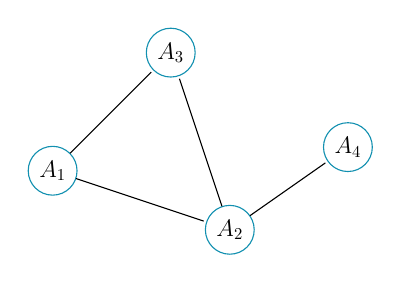
\begin{tikzpicture}	

      \tikzstyle{every edge}=[-,>=stealth',shorten >=1pt,auto,thin,draw]
		\node[observed] (A1) at (0*\edgeunit, 0*\edgeunit) {$A_1$};
		\node[observed] (A2) at (1.5*\edgeunit, -0.5*\edgeunit) {$A_2$};
		\node[observed] (A3) at (1*\edgeunit, 1*\edgeunit) {$A_3$};
		\node[observed] (A4) at (2.5*\edgeunit, 0.2*\edgeunit) {$A_4$};
		\path (A1) edge [] (A2)
        (A1) edge [] (A3)
        (A2) edge [] (A3)
        (A2) edge [] (A4);
	\end{tikzpicture}\\
\end{column}
\begin{column}{0.5\linewidth}
	\begin{itemize}
	\item Connected: all variables are dependant \bigskip
	\item \emphase{Markov property} : G encodes the conditional independences\\\bigskip
	 e.g. $A_4 \independent (A_1, A_3) \: |A_2$ \vspace{0.2cm}
\end{itemize}
\end{column}
\end{columns}
\begin{center}
 \only<1>{   \[ p(A_1, \dots, A_p) \propto \prod_{C \in \Ccal_G} \psi_C(A_C) \]
  where $\Ccal_G =$ set of maximal cliques of $G$.}
  \only<2>{ Here:  \[ P(A) \propto \psi_{1}(A_1,A_2,A_3) \; \psi_{2}(A_2,A_4) \]}
\end{center}
\end{frame}

%%%%%%%%%%%%%%%%%%%%%%%%%%%%%%%%%%
\begin{frame}{\textit{Gaussian Graphical Models} (GGM)}
 \vspace{-1cm}
 $$Y=(Y_1,...,Y_d) \sim \mathcal{N}_d(0,\Omega^{-1})$$\\
 \vspace{0.3cm}
 
 The factorization is straightforward:
$$p(y) \propto \prod_{j,k : \emphase{\omega_{jk} \neq 0 }} exp(-y_j \omega_{jk} y_k /2)  $$
\pause
\vspace{-1cm}
 \begin{columns} 
 \begin{column}{0.5\linewidth}

 \begin{flushright}
\[\Omega=
\left(
\begin{array}{*{4}{c}}
* & * & * & 0\\
*& * & * & *\\
* & * & * & 0\\
0 & * & 0 & *
\end{array}
\right)
\]
 \end{flushright}
 \end{column}
 \begin{column}{0.05\linewidth}
\begin{center}
 $\Rightarrow$
\end{center}
\end{column}
 \begin{column}{0.45\linewidth}
 \begin{flushleft}
\vspace{0.8cm}
 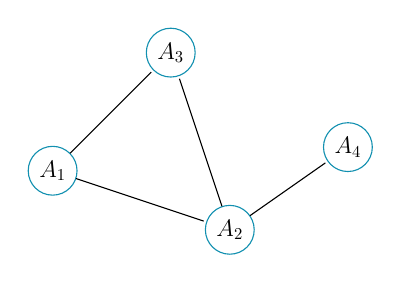
\begin{tikzpicture}
     
      \tikzstyle{every edge}=[-,>=stealth',shorten >=1pt,auto,thin,draw]
		\node[observed] (A1) at (0*\edgeunit, 0*\edgeunit) {$A_1$};
		\node[observed] (A2) at (1.5*\edgeunit, -0.5*\edgeunit) {$A_2$};
		\node[observed] (A3) at (1*\edgeunit, 1*\edgeunit) {$A_3$};
		\node[observed] (A4) at (2.5*\edgeunit, 0.2*\edgeunit) {$A_4$};
		\path (A1) edge [] (A2)
        (A1) edge [] (A3)
        (A2) edge [] (A3)
        (A2) edge [] (A4);

\end{tikzpicture}\\
\end{flushleft}
 \end{column}

\end{columns}
\end{frame}
%====================================================================
\begin{frame}{Missing actor}
$A_2$ is not observed:
 \begin{columns} 
 \begin{column}{0.5\linewidth}

 \begin{flushright}
 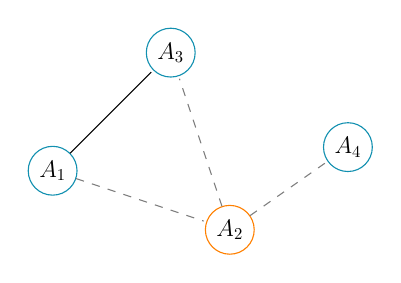
\begin{tikzpicture}
     
      \tikzstyle{every edge}=[-,>=stealth',shorten >=1pt,auto,thin,draw]
		\node[observed] (A1) at (0*\edgeunit, 0*\edgeunit) {$A_1$};
		\node[bigMissing] (A2) at (1.5*\edgeunit, -0.5*\edgeunit) {$A_2$};
		\node[observed] (A3) at (1*\edgeunit, 1*\edgeunit) {$A_3$};
		\node[observed] (A4) at (2.5*\edgeunit, 0.2*\edgeunit) {$A_4$};
		\path (A1) edge [gray,dashed] (A2)
        (A1) edge [] (A3)
        (A2) edge [gray,dashed] (A3)
        (A2) edge [gray,dashed] (A4);

\end{tikzpicture}\\
 \end{flushright}
 \end{column}
 \begin{column}{0.1\linewidth}
\begin{center}
\pause
 $\Longrightarrow$
\end{center}
\end{column}
 \begin{column}{0.4\linewidth}
 \begin{flushleft}
\vspace{0.8cm}
 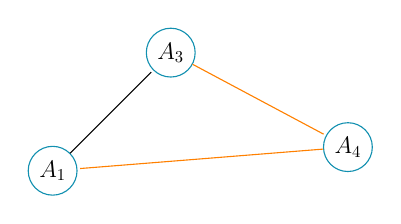
\begin{tikzpicture}
     
      \tikzstyle{every edge}=[-,>=stealth',shorten >=1pt,auto,thin,draw]
		\node[observed] (A1) at (0*\edgeunit, 0*\edgeunit) {$A_1$};
		%\node[observed] (A2) at (1.5*\edgeunit, -0.5*\edgeunit) {$A_2$};
		\node[observed] (A3) at (1*\edgeunit, 1*\edgeunit) {$A_3$};
		\node[observed] (A4) at (2.5*\edgeunit, 0.2*\edgeunit) {$A_4$};
		\path  (A1) edge [] (A3)
        (A3) edge [orange] (A4)
        (A4) edge [orange] (A1);

\end{tikzpicture}\\
\end{flushleft}
Spurious edges leading to wrong interpretation
 \end{column}
\end{columns}
\bigskip
\begin{center}
\only<3>{How to infer a missing actor in a network ?}
\only<4>{How to infer (a missing actor in) a network from abundance data?}
\end{center}
\end{frame}

%====================================================================
\section{Network inference}
\subsection{Abundance data}
\begin{frame}{Graphical model for abundance data}
$P\ell N$ model:
   \large{ $$ Y_{ij} \sim \mathcal{P}\big(\exp(\underbrace{o_{ij} + x_i^\intercal \thetab_j}_{\text{fixed}} + \underbrace{Z_{ij}}_{\text{random}})\big).$$} \normalsize 
     \pause
   \begin{itemize}
       \item classically \citep{AiH89}: $ \Zb_i \sim\mathcal{N}(0,\Omega^{-1})$ iid
       \item easy handling of multi-variate data, offsets and covariates
   \end{itemize}
   \bigskip
     \textit{GGM}: $\Omega$ encodes the \emphase{conditional dependency} structure.\\
   \pause
   \bigskip
   \citet{MRA20}: foster sparsity with a random spanning tree: $$Z|T \sim \mathcal{N}(0, \emphase{\Omega_T}^{-1}) $$
 Inference with an efficient variational EM algorithm.
\end{frame}

%====================================================================
\subsection{With trees}
\begin{frame}{Explore the space with trees}

\begin{columns}

\begin{column}{0.45\linewidth}
\only<1>{\begin{tabular}{c}
	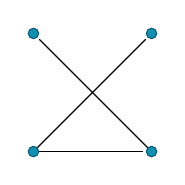
\begin{tikzpicture}
 \tikzstyle{every edge}=[-,>=stealth',shorten >=1pt,auto,thin,draw]
		\node[basic] (Z1) at (0*\edgeunit, 0*\edgeunit) {};
		\node[basic] (Z2) at (1*\edgeunit, 0*\edgeunit) {};
		\node[basic] (Z3) at (1*\edgeunit, 1*\edgeunit) {};
		\node[basic] (Z4) at (0*\edgeunit, 1*\edgeunit) {};
		\path (Z1) edge [] (Z2)
        (Z1) edge [] (Z3)
        (Z2) edge [] (Z4);
	\end{tikzpicture}\\
	\small{$p(T=t_1) = 0.12$}
\end{tabular}}
	   
\only<2>{\begin{tabular}{c}
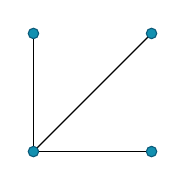
\begin{tikzpicture}
\tikzstyle{every basic}=[draw=none,text=black,scale=0.5,
      transform shape,circular drop shadow] 
		\node[basic] (Z1) at (0*\edgeunit, 0*\edgeunit) {};
		\node[basic] (Z2) at (1*\edgeunit, 0*\edgeunit) {};
		\node[basic] (Z3) at (1*\edgeunit, 1*\edgeunit) {};
		\node[basic] (Z4) at (0*\edgeunit, 1*\edgeunit) {};
		\path (Z1) edge [] (Z2)
        (Z1) edge [] (Z3)
        (Z1) edge [] (Z4);
		\end{tikzpicture} \\
		\small{$p(T=t_2) = 0.51$}
	   \end{tabular}}
	   
\only<3>{\begin{tabular}{c}
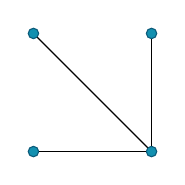
\begin{tikzpicture}
\tikzstyle{every basic}=[draw=none,text=black,scale=0.5,
      transform shape,circular drop shadow] 
		\node[basic] (Z1) at (0*\edgeunit, 0*\edgeunit) {};
		\node[basic] (Z2) at (1*\edgeunit, 0*\edgeunit) {};
		\node[basic] (Z3) at (1*\edgeunit, 1*\edgeunit) {};
		\node[basic] (Z4) at (0*\edgeunit, 1*\edgeunit) {};
		\path (Z1) edge [] (Z2)
        (Z2) edge [] (Z3)
        (Z2) edge [] (Z4); 
\end{tikzpicture}\\
		\small{$p(T=t_3) = 0.02$}
		\end{tabular}}
	   
\only<4>{\begin{tabular}{c}
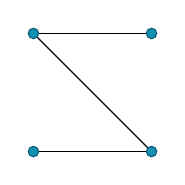
\begin{tikzpicture}
\tikzstyle{every basic}=[draw=none,text=black,scale=0.5,
      transform shape,circular drop shadow] 
		\node[basic] (Z1) at (0*\edgeunit, 0*\edgeunit) {};
		\node[basic] (Z2) at (1*\edgeunit, 0*\edgeunit) {};
		\node[basic] (Z3) at (1*\edgeunit, 1*\edgeunit) {};
		\node[basic] (Z4) at (0*\edgeunit, 1*\edgeunit) {}; 
		\path (Z1) edge [] (Z2)
        (Z3) edge [] (Z4)
        (Z2) edge [] (Z4);
\end{tikzpicture} \\
		\small{$p(T=t_4) = 0.3$}
\end{tabular}}

\only<5-6>{	 
\begin{tabular}{c}

\begin{tabular}{m{1cm} m{2cm}}
	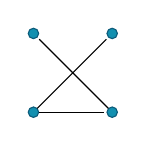
\begin{tikzpicture}
 \tikzstyle{every edge}=[-,>=stealth',shorten >=1pt,auto,thin,draw]
		\node[basic] (Z1) at (0*\smalledgeunit, 0*\smalledgeunit) {};
		\node[basic] (Z2) at (1*\smalledgeunit, 0*\smalledgeunit) {};
		\node[basic] (Z3) at (1*\smalledgeunit, 1*\smalledgeunit) {};
		\node[basic] (Z4) at (0*\smalledgeunit, 1*\smalledgeunit) {};
		\path (Z1) edge [] (Z2)
        (Z1) edge [] (Z3)
        (Z2) edge [] (Z4);
	\end{tikzpicture} &
	\small{$p(t_1) = 0.12$}
\end{tabular}\\

\begin{tabular}{m{1cm} m{2cm}}
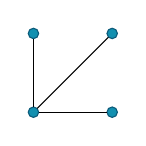
\begin{tikzpicture}
\tikzstyle{every basic}=[draw=none,text=black,scale=0.5,
      transform shape,circular drop shadow] 
		\node[basic] (Z1) at (0*\smalledgeunit, 0*\smalledgeunit) {};
		\node[basic] (Z2) at (1*\smalledgeunit, 0*\smalledgeunit) {};
		\node[basic] (Z3) at (1*\smalledgeunit, 1*\smalledgeunit) {};
		\node[basic] (Z4) at (0*\smalledgeunit, 1*\smalledgeunit) {};
		\path (Z1) edge [] (Z2)
        (Z1) edge [] (Z3)
        (Z1) edge [] (Z4);
		\end{tikzpicture} &
		\small{$p(t_2) = 0.51$}
	   \end{tabular}\\
	   
	   \begin{tabular}{m{1cm} m{2cm}}
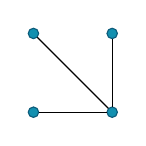
\begin{tikzpicture}
\tikzstyle{every basic}=[draw=none,text=black,scale=0.5,
      transform shape,circular drop shadow] 
		\node[basic] (Z1) at (0*\smalledgeunit, 0*\smalledgeunit) {};
		\node[basic] (Z2) at (1*\smalledgeunit, 0*\smalledgeunit) {};
		\node[basic] (Z3) at (1*\smalledgeunit, 1*\smalledgeunit) {};
		\node[basic] (Z4) at (0*\smalledgeunit, 1*\smalledgeunit) {};
		\path (Z1) edge [] (Z2)
        (Z2) edge [] (Z3)
        (Z2) edge [] (Z4); 
\end{tikzpicture}&
		\small{$p(t_3) = 0.02$}
		\end{tabular}\\

\begin{tabular}{m{1cm} m{2cm}}
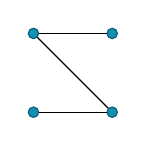
\begin{tikzpicture}
\tikzstyle{every basic}=[draw=none,text=black,scale=0.5,
      transform shape,circular drop shadow] 
		\node[basic] (Z1) at (0*\smalledgeunit, 0*\smalledgeunit) {};
		\node[basic] (Z2) at (1*\smalledgeunit, 0*\smalledgeunit) {};
		\node[basic] (Z3) at (1*\smalledgeunit, 1*\smalledgeunit) {};
		\node[basic] (Z4) at (0*\smalledgeunit, 1*\smalledgeunit) {}; 
		\path (Z1) edge [] (Z2)
        (Z3) edge [] (Z4)
        (Z2) edge [] (Z4);
\end{tikzpicture} &
		\small{$p(t_4) = 0.3$}
\end{tabular}\\

\Large{\textbf{.}}\\
\Large{\textbf{.}}\\
\Large{\textbf{.}}

\end{tabular}}
\end{column}

\begin{column}{0.45\linewidth}
\begin{center}
\only<6>{
Edge probabilities\footnotemark:\\
		\vspace{0.5cm}
		
\begin{tabular}{c}
		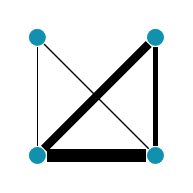
\begin{tikzpicture}
			\node[large] (Z1) at (0*\edgeunit, 0*\edgeunit) { };
		\node[large] (Z2) at (1*\edgeunit, 0*\edgeunit) { };
		\node[large] (Z3) at (1*\edgeunit, 1*\edgeunit) { };
		\node[large] (Z4) at (0*\edgeunit, 1*\edgeunit) { };
		\draw [line width=5pt] (Z1) -- (Z2); 
		\draw [line width=3pt] (Z1) -- (Z3); 
		\draw [line width=.5pt] (Z1) -- (Z4); 
		\draw [line width=2pt] (Z2) -- (Z3); 
		\draw [line width=.5pt] (Z2) -- (Z4); 
 %		\draw [line width=.5pt] (Z3) -- (Z4); 
		\end{tikzpicture}   \end{tabular}\\
		
		\vspace{0.5cm}
		
		$\displaystyle{\mathds{P}((j,k)\in T )= \sum_{\substack{t \in \mathcal{T}\\ (j,k)\in t}} p(t)}$
	
	   }
	   \end{center}
\end{column}

\end{columns}
\only<6>{
\footnotetext[1]{https://github.com/Rmomal/EMtree}}
\end{frame}

%====================================================================
\section{Missing actor}
\begin{frame}{More dimensions ?}
\begin{center}

\only<1>{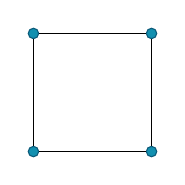
\begin{tikzpicture}
\tikzstyle{every basic}=[draw=none,text=black,scale=0.5,
      transform shape,circular drop shadow] 
		\node[basic] (Z1) at (0*\edgeunit, 0*\edgeunit) {};
		\node[basic] (Z2) at (1*\edgeunit, 0*\edgeunit) {};
		\node[basic] (Z3) at (1*\edgeunit, 1*\edgeunit) {};
		\node[basic] (Z4) at (0*\edgeunit, 1*\edgeunit) {}; 
		%\node[missing] (Z5) at (0.5*\edgeunit, 0.5*\edgeunit) {}; 
		\path (Z4) edge [] (Z3)
        (Z3) edge [] (Z2)
         (Z2) edge [] (Z1)
         (Z4) edge [] (Z1);
\end{tikzpicture}} 
\only<2>{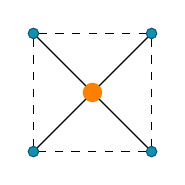
\begin{tikzpicture}
\tikzstyle{every basic}=[draw=none,text=black,scale=0.5,
      transform shape,circular drop shadow] 
		\node[basic] (Z1) at (0*\edgeunit, 0*\edgeunit) {};
		\node[basic] (Z2) at (1*\edgeunit, 0*\edgeunit) {};
		\node[basic] (Z3) at (1*\edgeunit, 1*\edgeunit) {};
		\node[basic] (Z4) at (0*\edgeunit, 1*\edgeunit) {}; 
		\node[missing] (Z5) at (0.5*\edgeunit, 0.5*\edgeunit) {}; 
		\path (Z5) edge [] (Z1)
        (Z5) edge [] (Z2)
        (Z5) edge [] (Z4)
        (Z5) edge [] (Z3)
        (Z4) edge [dashed] (Z3)
        (Z3) edge [dashed] (Z2)
         (Z2) edge [dashed] (Z1)
         (Z4) edge [dashed] (Z1);
\end{tikzpicture}} \\
\end{center}
\only<2>{
\begin{itemize}
\item Unobserved species
\item Unobserved covariate ?
\end{itemize}}

\bigskip\bigskip

\only<2>{Gaussian case: \citet{genevieve}}
\end{frame}

%====================================================================

\begin{frame}{Graphical model with missing actors}
\begin{columns}
\begin{column}{0.3\linewidth}
\begin{center}
\begin{tikzpicture}	
      \tikzstyle{every edge}=[-,>=stealth',shorten >=1pt,auto,thin,draw]
		\node[rectangle] (A1) at (0*\edgeunit, 2*\edgeunit) {$T$};
		\node[rectangle] (A2) at (0*\edgeunit, 1*\edgeunit) {$\Zb$};
		%\node[rectangle] (A3) at (1.25*\edgeunit, 1*\edgeunit) {$\Zb_H$};
		\node[rectangle] (A4) at (0*\edgeunit, 0*\edgeunit) {$\Yb$};
		\path (A1) edge [] (A2)
       % (A1) edge [] (A3)
     %   (A2) edge [] (A3)
        (A2) edge [] (A4);
	\end{tikzpicture} \\
	
	$$vBIC_0 = \mathcal{J}_0(\Yb) - \frac{D}{2}\log(n) $$
\end{center}
\end{column}

\begin{column}{0.65\linewidth}
\pause
\begin{center}
\begin{tikzpicture}	
      \tikzstyle{every edge}=[-,>=stealth',shorten >=1pt,auto,thin,draw]
		\node[rectangle] (A1) at (0.625*\edgeunit, 2*\edgeunit) {$T$};
		\node[rectangle] (A2) at (0*\edgeunit, 1*\edgeunit) {$\Zb_O$};
		\node[rectangle] (A3) at (1.25*\edgeunit, 1*\edgeunit) {$\Zb_H$};
		\node[rectangle] (A4) at (0*\edgeunit, 0*\edgeunit) {$\Yb$};
		\path (A1) edge [] (A2)
        (A1) edge [] (A3)
        (A2) edge [] (A3)
        (A2) edge [] (A4);
	\end{tikzpicture} \\
	
	$$vBIC_q = \mathcal{J}_q(\Yb) - \frac{D+2pq}{2}\log(n) $$
\end{center}
\end{column}
\end{columns}

\bigskip\bigskip
\end{frame}
%====================================================================
\subsection{Simulation data}
\begin{frame}{Results on a scale-free graph \emphase{\footnotesize{/!\textbackslash Work in progress /!\textbackslash }}}
\begin{center}
\includegraphics[width=4cm]{images/SFgraph}
\pause
\includegraphics[width=6cm]{images/Ghat}\\
\pause
\includegraphics[width=8.8cm]{images/precrec_missing.png}
\end{center}
\end{frame}
%====================================================================
\subsection{Illustration}
\begin{frame}{Barents fish data}
\begin{itemize}
\item Abundances of 30 species in 89 sites of the Barents sea
\item 4 available covariates (temperature, longitude, latitude, depth)
\end{itemize}

\bigskip\bigskip

Selection model criteria (no covariates):
$$vBIC_0 = 4431 \;\; \text{ vs. } \;\; vBIC_1 =8501$$

\end{frame}
%====================================================================

\begin{frame}{Inference with no covariates}

 \begin{center}
\only<1>{\includegraphics[width=6cm]{images/Barents_missing.png}}
\only<2>{\includegraphics[width=9cm]{images/R2_missing.png}}
 \end{center}
\only<1>{The inferred means of the missing actor are highly linked to the temperature}
\only<2>{Neighbors of the missing actor are also highly linked to the temperature}
 
\end{frame}
%====================================================================
\section{Conclusion}
\begin{frame}{Perspectives}
\begin{itemize}
\item Simulation study
\item Tests on spatialized data: 
\end{itemize}
\end{frame}
%====================================================================

\begin{frame}
\begin{center}
\Large{Thank you!}    
\end{center}

\bigskip
\bigskip

\small{
Contact :\\
\begin{description}
\item[email] raphaelle.momal@agroparistech.fr
\item[Web]Rmomal.github.io
\item[Twitter] @MomalRaphaelle\\
\end{description}}

\bigskip

\begin{center}
\footnotesize{Currently looking for a job opportunity!}
\end{center}
\end{frame}

%====================================================================
%====================================================================
%====================================================================
%====================================================================
%====================================================================
%====================================================================

\appendix
\backupbegin
\begin{frame}[allowframebreaks]
\bibliographystyle{apalike}
{\tiny
    \bibliography{biblio3}}
\frametitle{References}
%\bibliography{cellcite}
\end{frame}\backupend



\end{document}